
	Using any of the descriptions above, we have the space $\MM$ of flat $SU(2)$ connections on a compact connected Riemann surface $\Sigma$ of genus $g\geq 2$, which is a quasiprojective scheme with dimension $3g-3$. Furthermore, $\MM$ is equipped with the Atiyah-Bott symplectic form $\omega$, and there exists a line bundle $\LL$ over $\MM$ with curvature $2\pi i \omega$ \cite{quillen_determinants_1985}\cite{ramadas_comments_1989}. This is the data of a prequantum system to which we can apply geometric quantization.
	
	Jeffrey and Weitsman describe this quantization following an approach of \cite{weitsman_real_1992}, which is for a compact symplectic manifold $(M,\omega)$ and line bundle $\LL$, using a real polarization of $M$. A real polarization of $M$ is a map $\pi:M\to B$ onto a manifold of half dimension, such that $\omega|_{\pi^{-1}(b)} =0$ for all $b\in B$. Supposing $\pi:M\to B$ is also a fibration, there will be a finite set of \textit{Bohr-Sommerfeld points} $b_i$ for which $\LL$ restricted to the fibers $L_{b_i}$ of $\pi$ possesses global covariant constant sections. Denote $J_\pi$ denote the sheaf of sections of $\LL$ which are covariant constant along the fibres of $\pi$. Then the quantization of a prequantum system $(M,\omega,\LL)$ is the vector space
	\begin{equation}
		\mathcal{H} = \bigoplus_{i=0}^{\dim M} H^i(M,J_\pi).
	\end{equation}
	It is the dimension of $\mathcal{H}$ which we hope to compute. If $B_s$ is the set of all Bohr-Sommerfeld points, and for each $b\in B_s$ $S_b$ is the space of global covariant constant sections of $\LL|_{\pi^{-1}(b)}$, then Sniatycki (cite) proves that there is a natural isomorphism:
	\begin{equation}
		\mathcal{H} \cong \bigoplus_{b\in B_s} S_b.
	\end{equation}
	Since each $S_b$ is one dimensional, counting $\dim \mathcal{H}$ boils down to counting the Bohr-Sommerfeld points. 
	
	In this case, the above theorem does not apply because $\MM$ is not a smooth manifold and the polarisation we will describe is not a fibration. Sniatycki's theorem simply provides inspiration for investigating the Bohr-Sommerfeld set in $\MM$, and Jeffrey and Weitsman show that Bohr-Sommerfeld fibres are associated to marked trivalent graphs satisfying the quantum Clebsch-Gordan conditions, and the number of such graphs is called the \emph{Verlinde dimension}, counted by the \emph{Verlinde formula} \cite[Thm. 8.1]{jeffrey_bohr-sommerfeld_1992}.
	
\section{Polarisation of the Moduli Space}	
	As before, let $\Sigma$ be a compact Riemann surface and $\MM$ the moduli space of flat $G=SU(2)$ connections on $\Sigma$. Following Jeffrey and Weitsman, we describe an action of $T^{3g-3}$ on $\MM$. Let $C$ be a closed oriented curve in $\Sigma$ and pick a basepoint $y\in C$. We can define a function $\tilde{f}_C:\cA \to \mathbb{R}$ by 
	\begin{equation}
		\tilde{f}_C(A) = \frac{1}{2}\text{hol}_C(A),
	\end{equation}
	where hol$_C(A)$ means the holonomy of $A$ around $C$ from $y$ to $y$. Since the holonomy is $\cG$ invariant, this passes to $f_C:\MM \to \mathbb{R}$. $\Sigma$ admits a decomposition into \textit{trinions} or \textit{pairs of pants}, which are copies of a disc with two holes:
	\begin{equation}
		D = \{z \in \mathbb{C}~|~ |z|\leq 2 \} - \{z~|~|z-1|<1/2\}\cup \{z~|~ |z+1| < 1/2\},
	\end{equation}
	with marked points on the boundary of $D$. 

	\begin{figure}[h]
		\centering
		\subfloat[][Example: $g=2$.]{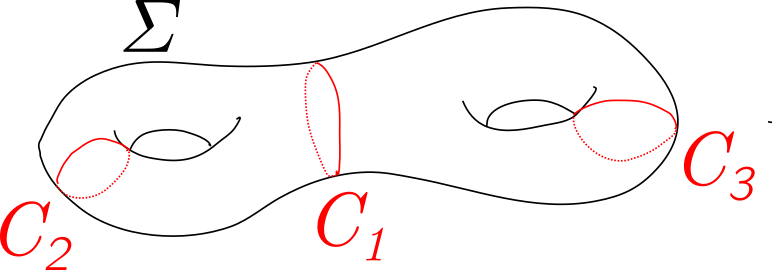
\includegraphics[width=0.5\linewidth]{genus2.png}\label{fig:genus2}}
		\subfloat[][General decomposition for $g\geq 3$.]{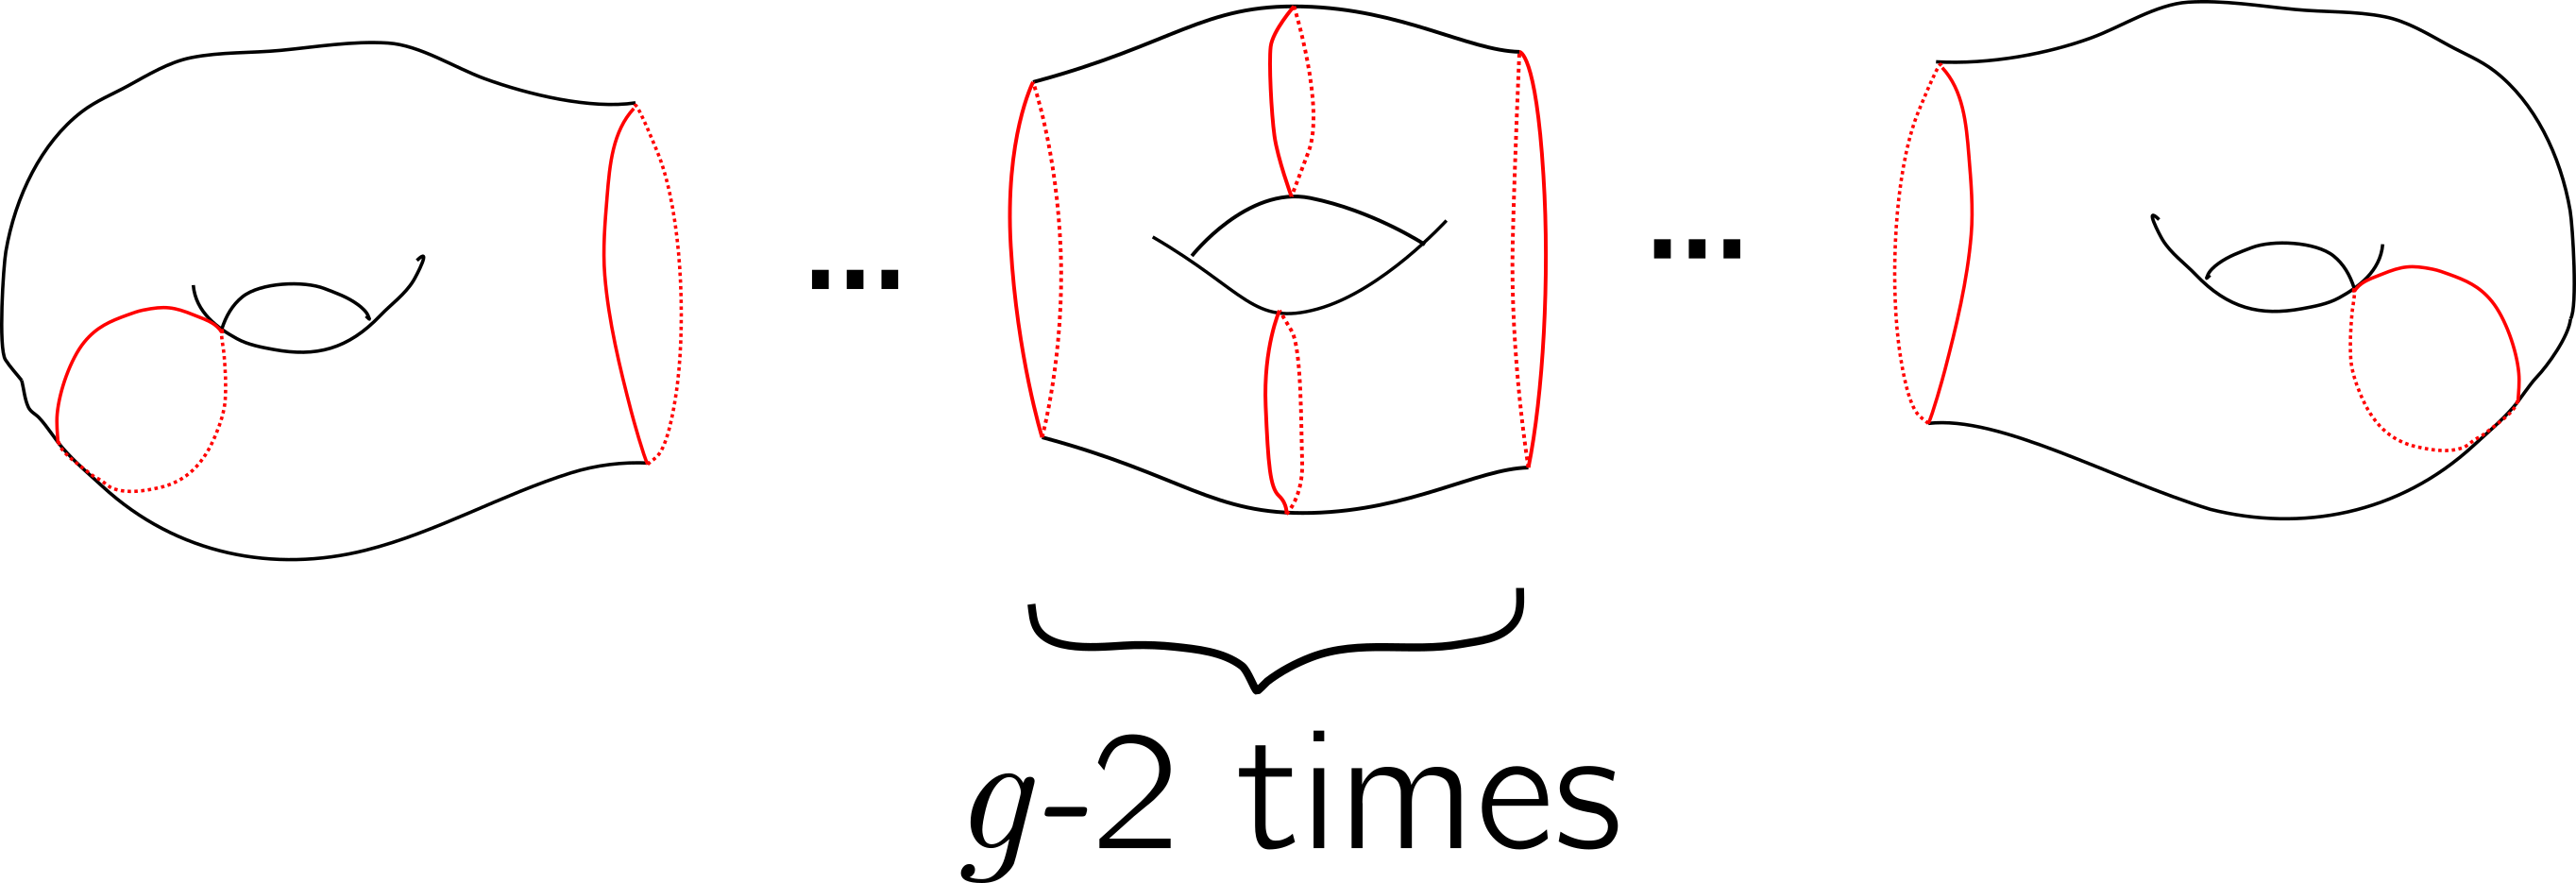
\includegraphics[width=0.5\linewidth]{genusg.png}\label{fig:genusg}}
		\caption{Decomposition of a surface $\Sigma$ into $2g-2$ trinions. }
		\label{fig:torusdecomp}
	\end{figure}

	Suppose we are given such a decomposition of $\Sigma$ into $2g-2$ trinions $D_\gamma$, $\gamma\in\{1,2,...,2g-2\}$, joined along their boundaries and with the marked points on the boundaries coinciding for any trinions with non-trivial intersection. Then the boundary circles of $D_\gamma$ give a collection $C_i$, $i\in\{1,2,...,3g-3\}$ of closed oriented curves in $\Sigma$ for which we get corresponding functions $f_i = f_{C_i}:\MM \to \mathbb{R}$ using the above definition. Since these functions are the trace of $SU(2)$ matrices, they can be described by cosine of angles $\theta_i$,
	\begin{equation}
		\theta_i(A) = \cos^{-1}(f_i(A)),
	\end{equation}
	where $\theta_i$ is taken to lie in $[0,\pi]$. This defines a map $\theta = (\theta_1,...,\theta_{3g-3}):\MM \to \mathbb{R}^{3g-3}$. These $\theta_i$ are smooth on $U_i := \theta_i^{-1}(0,\pi) \subset \MM$, which is open and dense. Thus, the Hamiltonian flows of each $\theta_i$ are defined on $\MM^{s} = \bigcap_{i=1}^{3g-3} U_i \subset \MM$. These Hamiltonian flows are periodic with constant period, which means they induce a torus action on $\MM^{s}$. Explicitly, if we let $X_i$ denote the Hamiltonian vector field of $\theta_i$, defined by
	\begin{equation}
		\iota_{X_i}\omega = d\theta_i,
	\end{equation}
	and let $e^{tX_i}$ be the corresponding vector field flow, then the action is given by $g = (\alpha_1,...,\alpha_{3g-3}) \in T^{3g-3}$ acts by
	\begin{equation}
		A \to e^{\alpha_1 X_1 + ... + \alpha_{3g-3}X_{3g-3}}A.
	\end{equation}
	 The Lie algebra of $T^{3g-3}$ is $
	\mathbb{R}^3$ and we interpret $\theta(A)$ as being dual by $\langle \theta, X \rangle = \sum \theta_i X_i$. Then
	\begin{equation}
		d\left(\langle \theta(A),X\rangle\right) = d\sum\theta_i X_i = \sum X_i d\theta_i = \iota_{X}\omega,
	\end{equation}
	which means $\theta$ is the moment map for the torus action. These functions $f_i$ also give us a real polarization of $\MM$. Let $B \subset \mathbb{R}^{3g-3}$ be the image of the $f_i$,
	\begin{equation}
		B = \{(f_i(E),...,f_{3g-3}(E))~|~ E \in \MM\},
		\label{e:B-def}
	\end{equation}
	then the fibers of the map $\pi = (f_1,...,f_{3g-3})$ foliate the smooth locus of $\MM$, and the generic fibre is a Lagrangian subvariety (cite J\&W). 
	
	Alternatively, one can describe the polarization using the picture of connections as representations of the fundamental group $\pi_1(\Sigma)$. First, a preliminary result. Let $T\subset SU(2)$ be a maximal torus.
	\begin{definition}
		A connection $A$ on $\Sigma^g$ is said to be \emph{adapted to a trinion decomposition} (a.t.d.) if there is a tubular neighbourhood $V_i \cong (-1,1)\times S^1$ of each boundary circle $C_i$ in the decomposition, such that in co-ordinates $(s,\theta)$ for $V_i$,
		\begin{equation}
			A|_{V_i} = X_i d\theta, 
		\end{equation}
		where $X_i$ is a constant element in $\mathfrak{t} = \text{Lie}(T)$.
	\end{definition}
	\begin{theorem}
		\label{t:atd-thm}
		For all $y\in \pi^{-1}(b)$, there exists an adapted to trinion decomposition connection $A$ in the gauge equivalence class $y$.
	\end{theorem}
	\begin{proof}
	First, any boundary circle $C$ in a trinion decomposition has tubular neighbourhood $V$ and co-ordinates $(s,\theta)$ in which the connection $y$ is written:
	\begin{equation}
		y = R(s,\theta)d\theta + S(s,\theta)ds,
	\end{equation}
	for some $R,S \in C^\infty(\Sigma, \mathfrak{su}(2))$. Then the desired gauge transformation by $g\in \cG$ is given by
	\begin{equation}
		g\cdot y = g^{-1}(Rd\theta + Sds)g + g^{-1}dg.
	\end{equation}	
	Let $g=Ce^{R(s,\theta)\theta}e^{-S(s,\theta)s}$. Then 
	\begin{equation}
		g^{-1}dg = g^{-1}(Rd\theta-Sds)g
	\end{equation}
	and therefore
	\begin{equation}
		g\cdot y = 2g^{-1}R(s,\theta)g~d\theta = 2C^{-1}e^{S(s,\theta)s}e^{-R(s,\theta)\theta} R(s,\theta)e^{R(s,\theta)\theta}e^{-S(s,\theta)s}C~d\theta.
	\end{equation}
	Now one can compute the partial derivatives to see that
	\begin{equation}
		\tilde{X} := e^{S(s,\theta)s}e^{-R(s,\theta)\theta} R(s,\theta)e^{R(s,\theta)\theta}e^{-S(s,\theta)s}
	\end{equation} 
	is a constant in $\mathfrak{g}$. We finally choose $C$ to diagonalize $\tilde{X}$ and let $X:= 2C^{-1}\tilde{X}C \in \mathfrak{t}$.
	
	Repeating this process for each boundary circle $C_i$ in our decomposition gives a set of local gauge transformations $g_i$ on each $V_i$ which we can patch together with smooth bump functions to get a global gauge transformation $g$ for which $A:=g\cdot y$ is adapted to trinion decomposition.
	\end{proof}
	
	This lets us define subgroups of $G=SU(2)$, which correspond to stabilizers of flat connections. Suppose $A$ is an a.t.d connection. Then the stabilizer of $A|_{C_i}$ in $\cG(C_i) = \Hom(C_i, G)$ consists of constant maps, and can thus be identified with a subgroup $H_i$ in $G$. If $\theta_i(A) \in \{0,\pi\}$, then $\text{hol}_{C_i}(A) = \pm\text{Id}$ and so $H_i = G$. Otherwise, $H_i = T$. 
	
	We can describe the fibre $\pi^{-1}(b)$ using these subgroups. Suppose $A$ is a.t.d. and $[A] \in \pi^{-1}(b)$. Let $\tau_i \in H_i$ for each circle $C_i$, $i\in (1,2,...,3g-3)$. Then define the map
	\begin{equation}
		\label{e:psiA}
		\psi_A : \prod_{i=1}^{3g-3} \to \pi^{-1}(b)
	\end{equation}
	as follows. Denote the trinions composing $\Sigma$ as $D_{\gamma}$, $\gamma\in{1,2,...,2g-2}$. For any circle $C_i$, let $D_{\gamma(i)}$, $D_{\gamma'(i)}$ be the trinions on either side. For $\tau=(\tau_1,\tau_2,...,\tau_{3g-3})$, choose a collection of maps $\zeta_\gamma : D_\gamma \to g$ such that for every $C_i$, $\zeta_{\gamma(i)}$ and $\zeta_{\gamma'(i)}$ are constant on a tubular neighbourhood of $C_i$, and such that
	\begin{equation}
		\zeta_{\gamma(i)}|_{C_i} = \tau_i \zeta_{\gamma'(i)}|_{C_i}.
	\end{equation}
	Here, adopt the convention that the orientation of the tubular neighbourhood is $v\wedge w$, where $w$ is tangent to the oriented circle $C_i$ and $v$ is transverse to $c_i$ and pointing \textit{into} $D_{\gamma(i)}$, thus away from $D_{\gamma'(i)}$.
	
	Now we define a connection $A_\tau$ on $\Sigma$ by defining $A_\tau$ on each trinion: $A_\tau|_{D_\gamma} := \zeta_\gamma \circlearrowright A|_{D_\gamma}$. Finally define $\psi_A(\tau) = [A_\tau]$. Next we ask, for $\tau,\tau' \in \prod_{i=1}^{3g-3} H_i$, when are $A_\tau$ and $A_{\tau'}$ gauge equivalent? 
	
	Let $J_\gamma$ be the stabilizer of $A|_{D_\gamma}$ under $\cG|_{D_\gamma} = \Hom(D_\gamma,G)$. Since $A$ is a.t.d., this also consists of constant maps. $J_\gamma = Z(G) = \{\pm \text{Id}\}$ if the holonomy is an irreducible representation of $SU(2)$, and otherwise $J_\gamma =T$ (resp $G$) if the holonomy reduces to $T$ (resp $Z(G)$).  
	
	Jeffrey and Weitsmasn give us the following lemma and theorem:
	\begin{theorem}
		If $\tau,\tau'$ are in $\prod_{i=1}^{3g-3} H_i$, then $[A_\tau] = [A_{\tau'}]$ if and only if there is a set of gauge transformations $\Phi_\gamma:D_\gamma \to G$ such that:
		\begin{enumerate}
			\item $\Phi_\gamma \in J_\gamma$ for all $\gamma$.
			\item For each boundary circle $C_i$, we have
			$$
				\Phi_{\gamma'(i)}|_{C_i} \tau_i = \tau_i' \Phi_{\gamma(i)}|_{C_i}.
			$$
		\end{enumerate}
	\end{theorem} 
	\begin{theorem}
		The map $\psi_A:\prod_i H_i \to \pi^{-1}(b)$ is surjective and the group $\prod_\gamma J_\gamma$ has a natural action on $\prod_i H_i$ so that
		\begin{equation}
			\pi^{-1}(b) = \left(\prod_i H_i\right)/\left(\prod_\gamma J_\gamma\right).
		\end{equation}
	\end{theorem}
	\begin{proof}
		jeffrey and weitsman page 600
	\end{proof}

\section{Moduli of Connections on a Trinion}
 	Now we've seen that the space $\MM$ can be constructed by glueing together connections defined along a trinion decomposition, so the natural question is what the space of connections on a trinion $D$, denoted $\MM(D)$, looks like. The space $\MM(D)$, like $\MM$, can be described the quotient of representations of the fundamental group into $G$ under conjugation by $G$. For a trinion, 
	\begin{equation}
		\pi_1(D) = \left\{
		[C_1], [C_2], [C_3] ~|~ [C_1][C_2][C_3]  =1
		\right\},
	\end{equation}
	where $C_i$ are the three boundary curves of the trinion. We can again define the holonomy angle functions, first letting $\tilde{\theta_i}:\Hom(\pi_1(D),G) \to [0,\pi]$ be
	\begin{equation}
		\label{e:thetacoords}
		\tilde{\theta_i}(\rho) = \cos^{-1}\left(\frac{1}{2}\Tr(\rho[C_i])\right),
	\end{equation}
	and these maps will descend under the quotient by $G$ to maps $\theta_i:\MM(D)\to [0,\pi]$. Then Jeffrey and Weitsman prove:
	\begin{theorem}
		The map $\theta = (\theta_1, \theta_2, \theta_3):\MM(D)\to[0,\pi]^3$ sends $\MM(D)$ bijectively to the set satifying the inequalities
		\begin{equation}
			|\theta_1 - \theta_2| \leq \theta_3 \leq \min(\theta_1 + \theta_2, 2\pi - (\theta_1 + \theta_2)).
			\label{e:trinion-ineqs}
		\end{equation}
		Remark that this set is a 3D simplex (insert figure?)
	\end{theorem}
	\begin{proof}
		J\&W prop 3.1
	\end{proof}
	Using this result, and the gluing process described in the last section, the image of $\MM$ under the holonomy angles $\theta_1,...,\theta_{3g-3}$ are the values satisfying the inequalities (\ref{e:trinion-ineqs}) on every trinion. Applying a theorem of Guillemin and Steinberg (cite) to this case, one obtains:
	\begin{theorem}
		\label{t:torusfibres}
		Suppose $x\in \pi(\MM) \subset B$ (defined in eqn. \ref{e:B-def}) Then
		\begin{itemize}
			\item The Hamiltonian vector fields corresponding to the functions $\theta_i$ are linearly independent on the fibre $\pi^{-1}(x)$, if and only if $x$ is a point where all the inequalities (\ref{e:trinion-ineqs}) are strict.
			\item In general, the number of linearly independent Hamiltonian vector fields on the fibre $\pi^{-1}(x)$ is equal to $3g-3-s$, where $s$ is the number of independent linear equations out of the following satisfied by $\theta(x)$:
				\begin{align*}
					\theta_{i_{\sigma(1)}(\gamma)}(x) + \theta_{i_{\sigma(2)}(\gamma)}(x)-\theta_{i{_\sigma(3)}(\gamma)}(x)&=0,\\
					\theta_{i_1(\gamma)}(x) + \theta_{i_2(\gamma)}(x) + \theta_{i_3(\gamma)}(x) = 2\pi.
				\end{align*}
			where $\sigma:{1,2,3}\to{1,2,3}$ is any cyclic permutation. These inequalities correspond to $(\ref{e:trinion-ineqs})$.
		\end{itemize}
	\end{theorem}
	Furthermore
	\begin{lemma}
		Let $x\in \MM(D)$ and let $\theta(x)$ be the holonomy angles of $x$ around the three boundary curves of $D$. Then $x$ corresponds to a conjugacy class of reducible representations of $\pi_1(D)$ if and only if at least one of the equations (\ref{e:theta-ineqs}) above is satisfied.
	\end{lemma}
	Motivated by this lemma, one defines \emph{interior triples} in $[0,\pi]^3$ to be those for which none of the equations is satisfied, i.e those on the interior of the simplex. These triples correspond to points in $\MM(D)$ which are conjugacy classes of irreducible representations of $\pi_1(D)$. Theorem \ref{t:torusfibres} tells us that the fibre $\pi^{-1}(x)$ is a torus if and only if $\theta(x)$ is an interior triple.
	\begin{theorem}
		Let $x\in B$ and let $A$ be a flat a.t.d. connection whose gauge equivalence class is in $\pi^{-1}(x)$. Further, assume that on every trinion the holonomy angles of $x$ is an interior triple. Then the fibre $\pi^{-1}(x)$ is identified with $T^{3g-3}/(\mathbb{Z}_2)^{2g-2}$ under the map $\psi_A$ defined in eqn. (\ref{e:psiA}).
	\end{theorem}
	Thus, the fibres corresponding to interior triples, which are the generic fibres, are tori of dimension $3g-3$. It is the non-generic fibres, corresponding to reducible points, which cause the result of Sniatycki to fail here.

	
	\section{Counting Bohr-Sommerfeld Points}
	With this real polarization of the moduli space, Jeffrey and Weitsman proceed to count the number of Bohr-Sommerfeld points \cite{jeffrey_bohr-sommerfeld_1992}. In this section we will lay out the results that we want to use going forward.
	
	\begin{definition}
		Let $(\MM,\omega)$ be a symplectic manifold with prequantum line bundle $\LL$ and polarisation $\pi:\MM\to B$. A point $b\in B$ is called a \emph{Bohr-Sommerfeld} point if $\LL|_{\pi^{-1}(b)}$ possess a one-dimensional family of global covariant constant sections.
	\end{definition}
	The quantization of a prequantum system is $\mathcal{H} = \bigoplus_{i=1}^{\dim M} H^i(M, \mathcal{J}_\pi)$, where $\mathcal{J}_\pi$ is the sheaf of sections of $\LL$ covariant constant along the fibres of $\pi$. Sniatycki's theorem \cite{sniatycki_cohomology_1977} proves that when the polarisation is a fibration, the dimension of $\mathcal{H}$ is given by the number of Bohr-Sommerfeld points. Although this result does not apply here, it still provides motivation for counting the Bohr-Sommerfeld points.
	
	For $\Sigma$ a connected compact Riemann surface of genus $g$, fix a trinion decomposition $\{D_\gamma\}$, and label the boundary loops of $D_\gamma$ as $C_{i_1(\gamma)}$, $C_{i_2(\gamma)}$ and $C_{i_3(\gamma)}$. We call a boundary loop $C_i$ \emph{separating} if removing it disconnects $\Sigma$. Recall the co-ordinates $\theta_i$ for the points $x\in \MM$ defined in equation $\ref{e:thetacoords}$. 
	\begin{theorem}[J\&W Thm 8.1]
		\label{t:bs-count}
		The set $P^{bs}$ of Bohr-Sommerfeld points in $B$ is given by the points $x\in B$ satisfying the conditions:
		\begin{enumerate}
			\item For each boundary circle $C_i$, $\theta_i(x) = \frac{\pi l_i}{k}$ for some $l_i \in \mathbb{Z}_k$, with $l_i$ even if $C_i$ is separating.
			\item For each trinion $D_\gamma$, $l_{i_1(\gamma)} + l_{i_2(\gamma)} + l_{i_3(\gamma)} \in 2\mathbb{Z}$.
		\end{enumerate}
	(what is $k$?)
	\end{theorem}
	From theorem \ref{t:torusfibres}, we know that $(\theta_1,...,\theta_{3g-3})$ is the image of a point $x\in B$ if and only if the conditions (\ref{e:trinion-ineqs}) are satisfied for the triple $(\theta_{i_1(\gamma)}, \theta_{i_2(\gamma)}, \theta_{i_3(\gamma)})$ corresponding to each trinion $D_\gamma$. We can represent a trinion decomposition as a trivalent graph, with a vertex for each trinion and an edge for each boundary circle. Therefore, a Bohr-Sommerfeld point gives a labelled trivalent graphs, where the integer $l_i$ is assigned the edge corresponding to boundary circle $C_i$. The set of Bohr-Sommerfeld points is bijective with labelled trivalent graphs whose labelling satisfy certain conditions. This picture gives the final result of Jeffrey and Weitsman:
	\begin{theorem}[J\& W Thm 8.3]
		Consider a fixed trinion decomposition of a compact connected Riemann surface $\Sigma$ of genus $g$. It gives rise to a trivalent graph, and a real polarisation of the moduli space $\MM$ of flat $SU(2)$ connections on $\Sigma$. There is one-to-one correspondence between the Bohr-Sommerfeld points of the polarisation and the set of integer labellings of the edges of the graph satisfying the conditions 1,2 in \ref{t:bs-count} and equation \ref{e:trinion-ineqs}.
	\end{theorem}
	Importantly, this theorem tells us that the Bohr-Sommerfeld points are counted inside the moment polytope defined by equation \ref{e:trinion-ineqs}. In the next section, we discuss the construction of a larger moduli space which is a smooth toric variety, allowing us to apply Sniatycki's theorem, but whose moment polytope agrees that that of $\MM$. This means the quantization of the larger moduli space has dimension given by this point-count; it will remain to show that the quantization of the larger moduli space agrees with that of $\MM$. 
	
	